\section{Versuchsaufbau}
\label{sec:Versuchsaufbau}

Dieser Versuch wird mit einer Apparatur, wie sie in 
Abbildung \ref{abb1} dargestellt ist, durchgeführt.
Dabei befindet sich eine Spektrallampe mit dem Material 
Cadmium (Cd) zwischen den Polen eines Elektromagneten, 
welcher ein Magnetfeld erzeugen kann, dessen Feldlinien 
transversal zu den elektromagnetischen Strahlen der 
Cd-Lampe verlaufen.
Ihr emittiertes Licht wird daraufhin durch ein Objektiv und 
eine Kondensorlinse auf einen Spalt gerichtet. Eine zweite 
Linse projeziert den Strahl danach auf ein Geradsichtprisma, 
welches die Eigenschaft hat, Licht nach seiner 
Wellenlänge separieren zu können. Jetzt kann es durch einen 
Polarisationsfilter nach seiner Polarisation und durch einen 
Spalt nach seiner Wellenlänge ausgewählt werden, sodass es 
schließlich auf eine Lummer-Gehrke-Platte \ref{LGP} abgebildet 
wird. Um eine vollständige Abbildung auf das Eintrittsfenster
der Platte und auf den davor verbauten Spalt zu ermöglichen, 
befinden sich zwischen Filter und Spalt, sowie zwischen 
Spalt und Lummer-Gehrke-Platte zwei weitere Linsen. 
Die Srahlen, die das Gehäuse um die Platte verlassen,
können schließlich mit einer Digitalkamera fotographisch 
festgehalten werden.

\begin{figure}
    \centering
    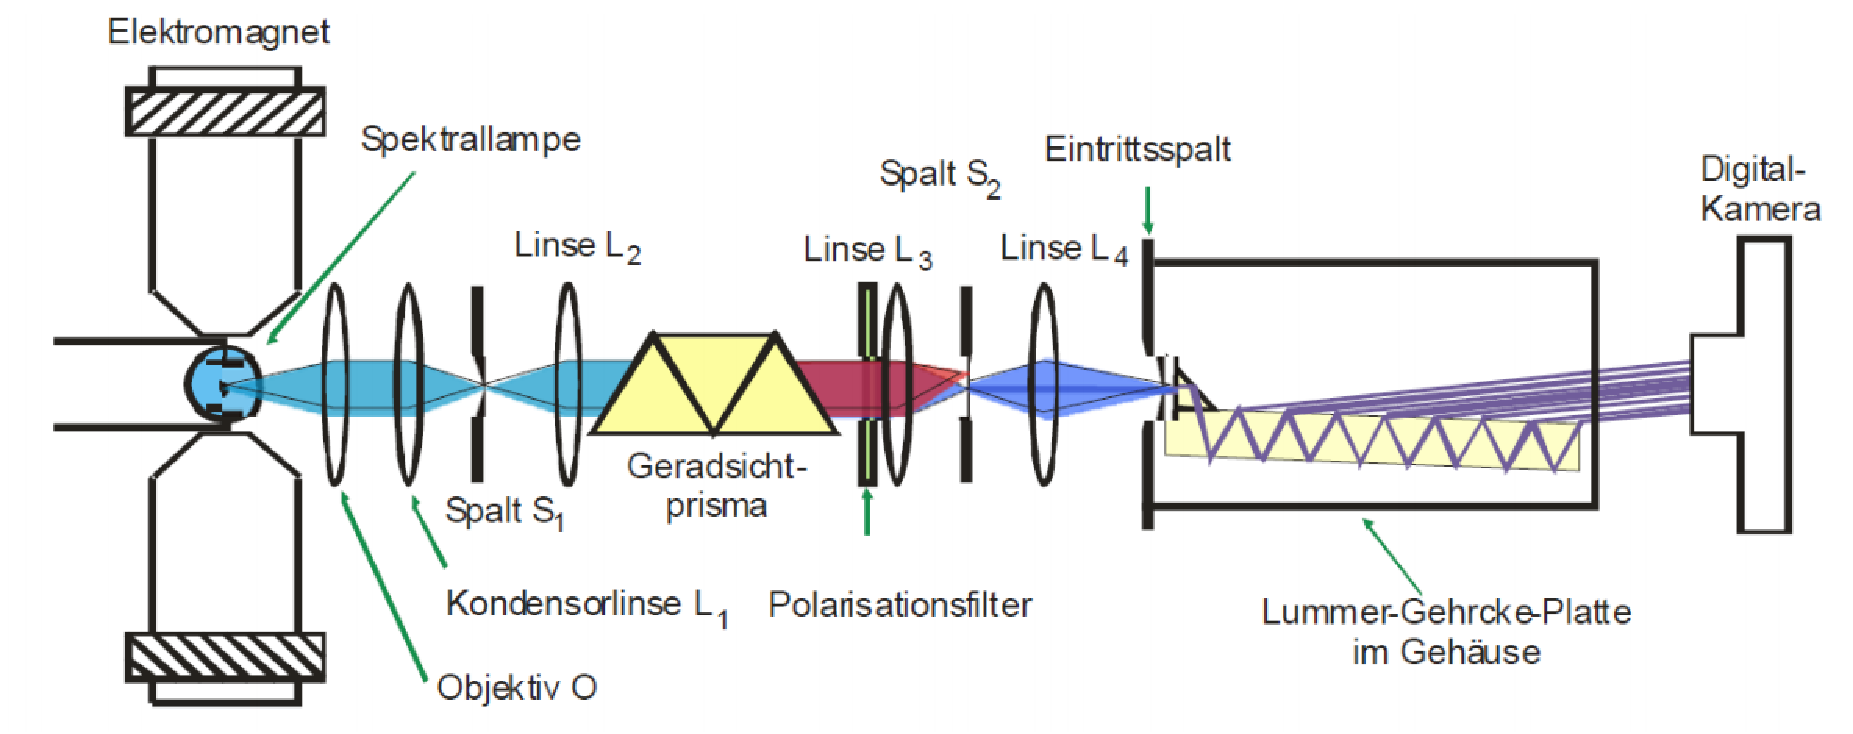
\includegraphics[width=0.7\textwidth]{figure/Aufbau.pdf}
    \caption{Diese Abbildung zeigt den schematischen Aufbau dieses Versuches \cite{sample}.}
    \label{abb1}
\end{figure}

\subsection{Die Lummer-Gehrke-Platte}
\label{LGP}

Eine Lummer-Gehrke-Platte besteht aus zwei planparallelen 
Platten, welche im Abstand $d$ voneinander befestigt sind.
Am Eintrittsfenster in den durch die Platten begrenzten Raum 
befindet sich ein Prisma. Parallel einfallendes Licht
wird durch das Prisma im Winkel $\beta$ auf eine der Platten 
gelenkt und an ihr reflektiert, sodass es im gleichen Winkel 
auf die andere Platte treffen kann. Auf diese Weise durchläuft 
ein Lichtstrahl die Lummer-Gehrke-Platte, wobei immer auch
ein Teil des Lichts an den Reflektionspunkten im Winkel $\alpha$ transmittiert wird \ref{abb2}.

\begin{figure}
    \centering
    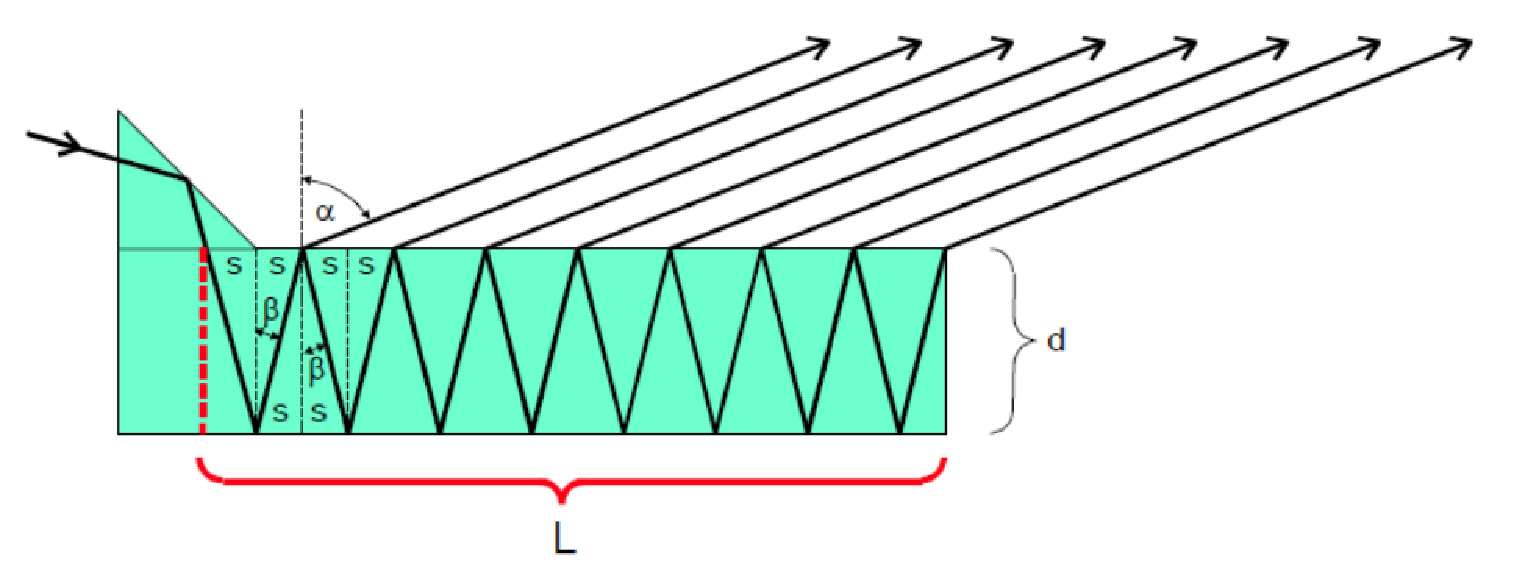
\includegraphics[width=0.6\textwidth]{figure/LGP.pdf}
    \caption{In dieser Abbildung ist die Reflektion und Transmission eines 
    Lichtstrahles in einer Lummer-Gehrke-Platte dargestellt.}
    \label{abb2}
\end{figure}

Zwischen den Transmissionsstrahlen herrscht genau dann 
konstruktive Interferenz, wenn die Bedingung

\begin{equation}
    2nd \cos(\beta) = m \lambda
    \label{eq1}
\end{equation}

gilt. $\lambda$ ist in dieser Gleichung die Wellenlänge des 
einfalllenden Lichtstrahles und $n$ der Brechungsindex der Platte, 
welcher durch 

\begin{equation}
    n = \frac{\sin(\alpha)}{\sin{\beta}}
    \label{eq2}
\end{equation}

gegeben ist. Einen weiteren Einfluss hat die Ordnungszahl der 
Interferenz, welche in Gleichung \ref{eq1} durch $m$
gegeben ist.\\
Für den Fall eines monochromatisch einfallenden 
Lichtstrahls ist der Gangunterschied der Interferenz von der
Breite der Wellenlänge des Lichtes. 
Das führt dazu, dass sich die Änderung der Wellenlänge an der 
Änderung des Abstandes der Interferezstreifen ablesen lässt.
Eine solche Änderung kann bspw. durch ein eingeschaltetes 
Magnetfeld am Elektromagneten \ref{abb1} erzeugt werden.\\
Das Dispersionsgebiet einer Lummer-Gehrke-Platte ist 
der Spektralbereich, für den eine Messung möglich ist. 
Um eine Überlagerung der Ordnungen zu vermeiden, sollten 
zwei Wellenlängen maximal auf eine Differenz von der 
Größe dieses Spektralbereiches aufgespalten werden. 
Für große Austrittswinkel $\alpha$ ist er durch 

\begin{equation}
    \Delta \lambda_{\symup{D}} = \frac{\lambda^2}{2d} \frac{1}{\sqrt{n^2 -1}}
    \label{eq:del_Lam}
\end{equation}

gegeben. Das Auflösungsvermögen einer Lummer-Gehrke-Platte ist 
neben ihr zugeordneten Eigenschaften, wie der Plattenlänge und 
dem Brechungsindex, auch von der Wellenlänge des Lichtes 
abhängig. Es kann über den folgenden Zusammenhang bestimmt 
werden:

\begin{equation}
    A = \frac{\lambda}{\delta \lambda} = \frac{L}{\lambda}(n^2 -1)
    \label{eq:del_A}
\end{equation}

Dieser Abschnitt wurde mit der Literaturangabe \cite{sample} erstellt.

\section{Versuchsdurchführung}
\label{sec:Versuchsdurchführung}

Die Versuchsdurchführung wird in vier Hauptaufgaben unterteilt.
Zunächst muss der Elektromagnet geeicht werden. Danach kann die 
Apparatur justiert werden und schließlich kann die Messung 
der Wellenlängenaufspaltung für rote und blaue Spektrallinien 
durchgeführt werden \cite{sample}.

\begin{enumerate}
    \item Eichung des Elektromagneten:
    \begin{itemize}
        \item Das B-Feld wird in Abhängigkeit des Feldstroms gemessen.
        \item Im Bereich von $\SI{0,45}{\ampere}$ bis $\SI{5,02}{\ampere}$
        werden 10 Wertepaare aufgenommen.
    \end{itemize}
    \item Justierung der Apparatur:
    \begin{itemize}
        \item Die Strahlung der Cd-Lampe wird mit Hilfe des ersten 
        Objektivs und der ersten Linse auf den ersten Spalt (siehe \ref{abb1})
        abgebildet.
        \item Die zweite Linse wird so eingestellt, dass der auf das Geradsichtprisma
        einfallende Strahl möglichst parallel ist. Es wird außerdem darauf geachtet, dass der 
        gesamte Strahl in das Prisma eindringen kann, sodass möglichst wenig 
        Strahlungsintensität für die Messung verloren geht.
    \end{itemize}
    \item Messung der Wellenlängenaufspaltung für rote Spektrallinien:
    \begin{itemize}
        \item Am zweiten Spalt kann eine Wellenlänge, in diesem Fall eine Rote,
        gewählt werden. Dafür wird mit der dritten Linse ein scharfes Bild am 
        zweiten Spalt erzeugt.
        \item Die vierte Linse wird so eingestellt, dass ein scharfes Bild von der Größe des 
        Eintrittsfensters auf die Lummer-Gehrke-Platte abgebildet wird.
        \item Am Polarisationsfilter wird der Übergang $\delta m= \pm,0$ mit B-Feld, sowie keine 
        Polarisation einmal mit und einmal ohne B-Feld eingestellt.
        Die Feldstromstärke beträgt bei diesen Messungen jeweils $\SI{5,02}{\ampere}$
        Die folgenden Stichpunkte werden für jede Porlarisationseinstellung einzeln durchlaufen.
        \item Wenn eine Aufspaltung der Zeeman-Linien zu erkennen ist, 
        werden sie mit einer Digitalkamera am Ende der Lummer-Gehrke-Platte
        aufgenommen.
    \end{itemize}
    \newpage
    \item Messung der Wellenlängenaufspaltung für blaue Spektrallinien:
    \begin{itemize}
        \item Die Einstellungen der Apparatur werden analog zur Messung der roten 
        Spektrallinien durchgeführt, wobei die Einstellungen am Polarisationsfilter variiert werden.
        \item Zunächst wird bei einer Feldstromstärke von $\SI{3,96}{\ampere}$ eine Messung der Übergänge
        $\delta m= \pm,0$ vorgenommen. Dann wird eine Messung ohne Polarisation, jedoch mit Magnetfeld 
        aufgenommen.
        \item Dieser Messvorgang wird für eine Feldstromstärke von $\SI{5,05}{\ampere}$ wiederholt.
    \end{itemize}
\end{enumerate}
